% !TeX root = ../main.tex

\section{Resultate}

\begin{frame}{Resultate {\scriptsize \cite[S.~101-102]{stenningHumanReasoningCognitive2008}}}
    \begin{itemize}
        \item jede Manipulation bringt (unterschiedlich gute) Verbesserung
        \item entsprechend Vorhersagen der Theorien, von denen Manipulationen abgeleitet wurden
        \item starke Evidenz für Zusammenhang zwischen Manipulationen und mentalen Vorgängen, auf die sie einwirken
    \end{itemize}
\end{frame}


\begin{frame}{Resultate {\scriptsize \cite[S.~101]{stenningHumanReasoningCognitive2008}}}
    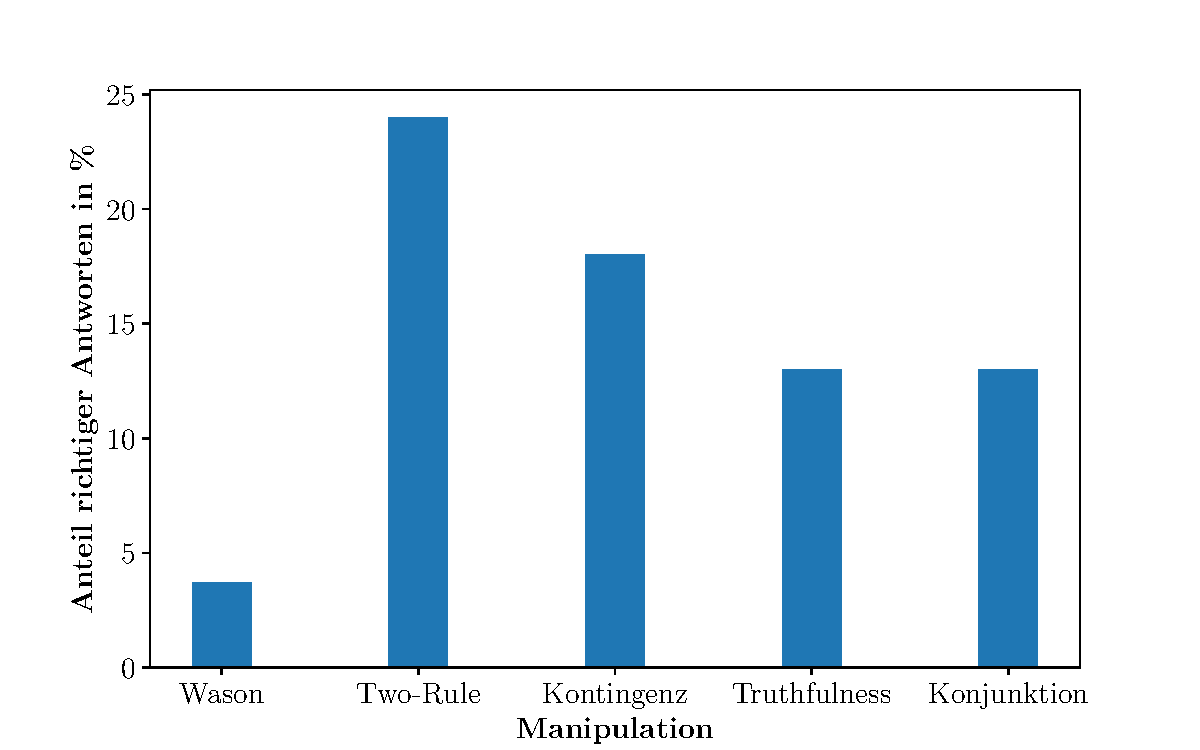
\includegraphics[width=\textwidth]{../plot/results_correct.pdf}
\end{frame}


\begin{frame}{Two-Rule Task {\scriptsize \cite[S.~102-104]{stenningHumanReasoningCognitive2008}}}
    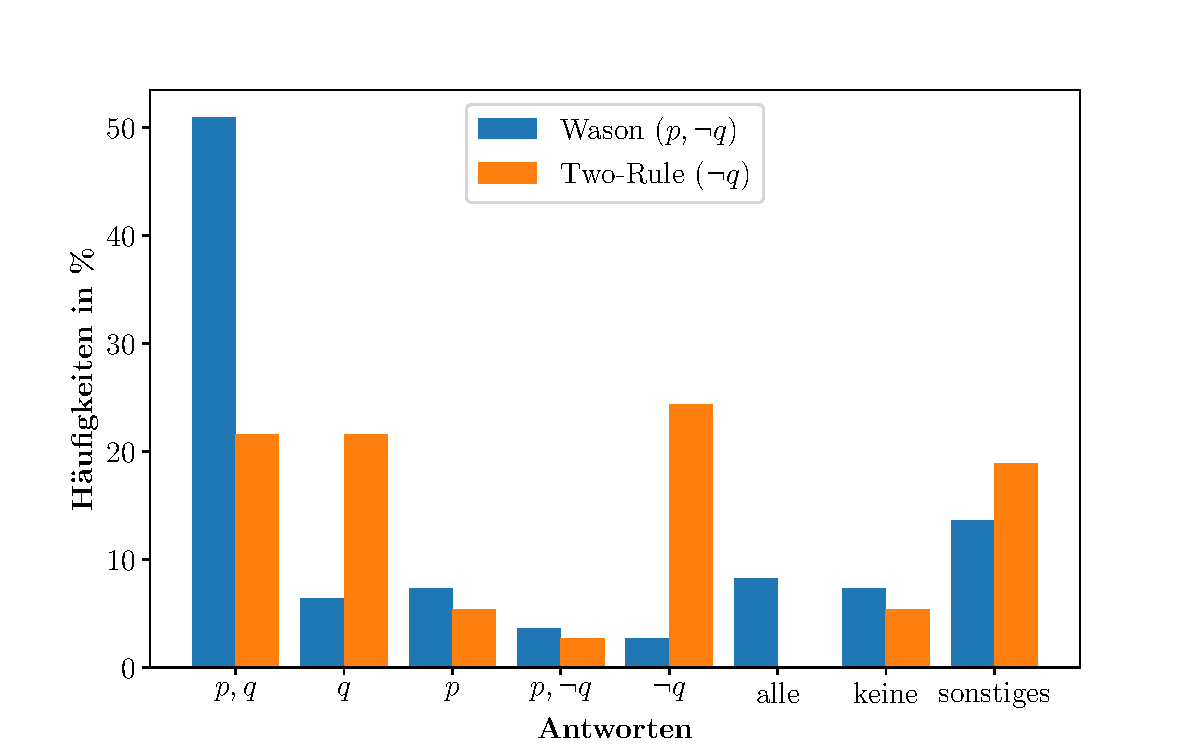
\includegraphics[width=\textwidth]{../plot/results_two_rule.pdf}
\end{frame}


\begin{frame}{Kontingenz {\scriptsize \cite[S.~109]{stenningHumanReasoningCognitive2008}}}
    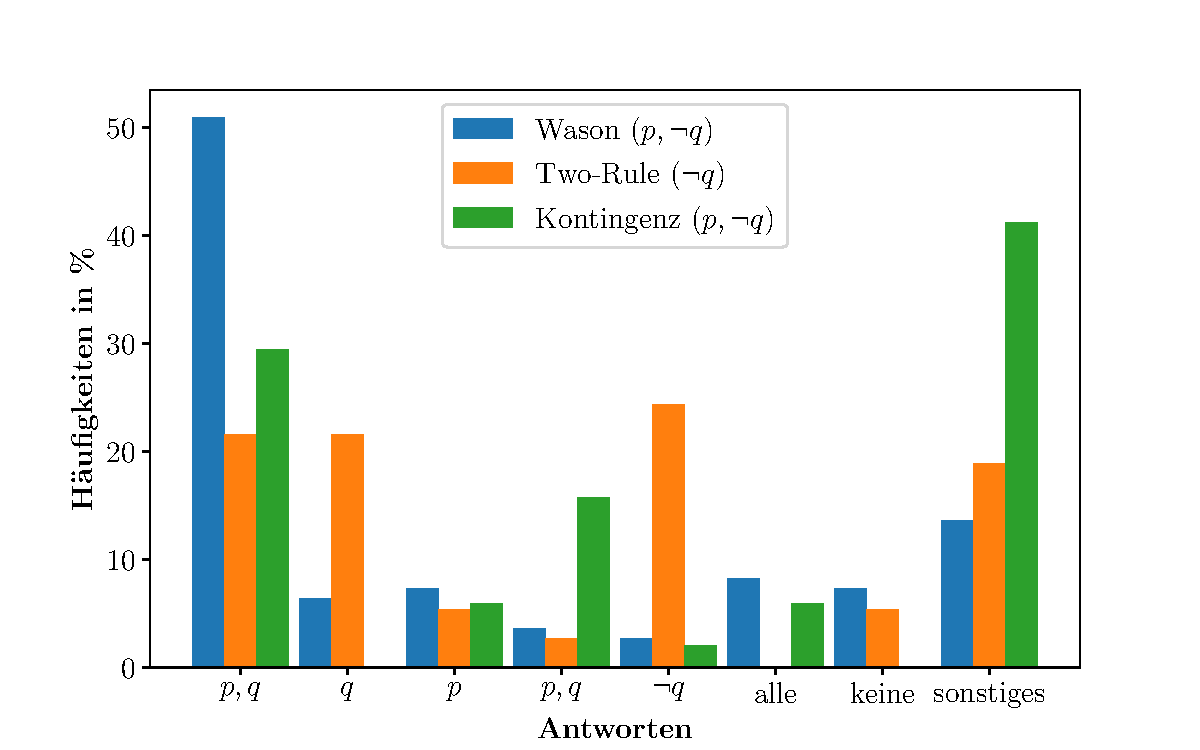
\includegraphics[width=\textwidth]{../plot/results_contingency.pdf}
\end{frame}


\begin{frame}{Truthfulness {\scriptsize \cite[S.~109]{stenningHumanReasoningCognitive2008}}}
    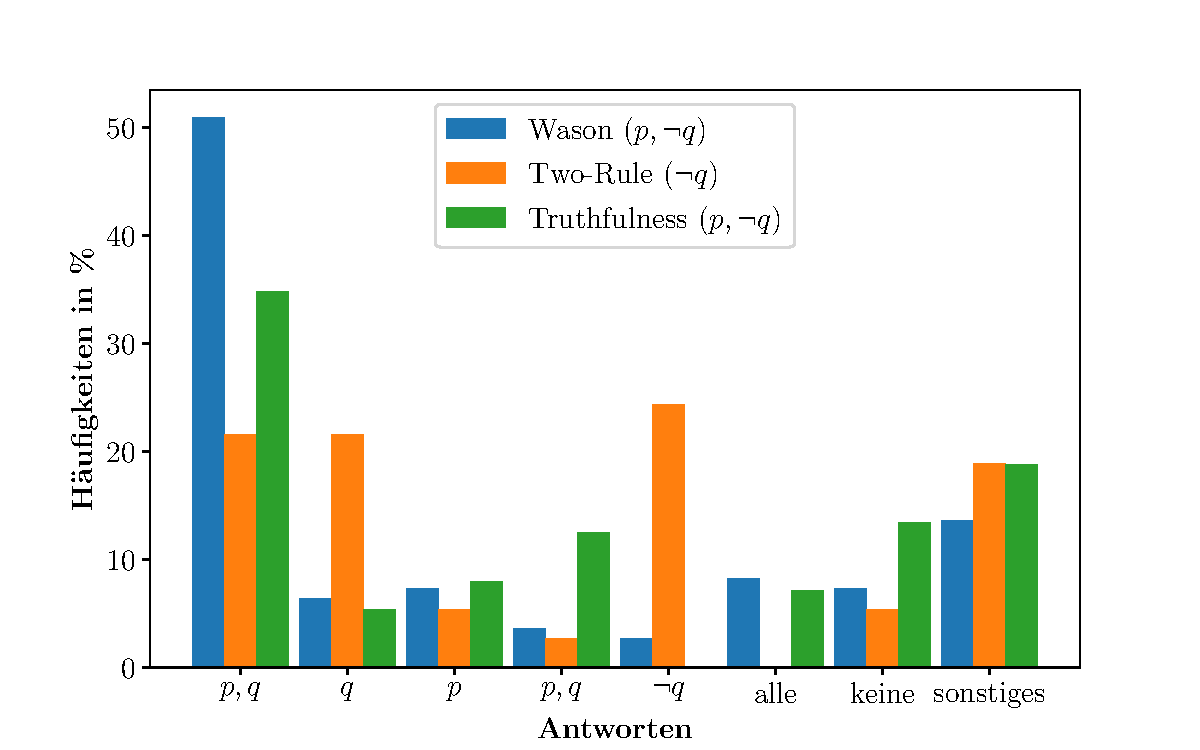
\includegraphics[width=\textwidth]{../plot/results_truthfulness.pdf}
\end{frame}


\begin{frame}{Konjunktion {\scriptsize \cite[S.~109]{stenningHumanReasoningCognitive2008}}}
    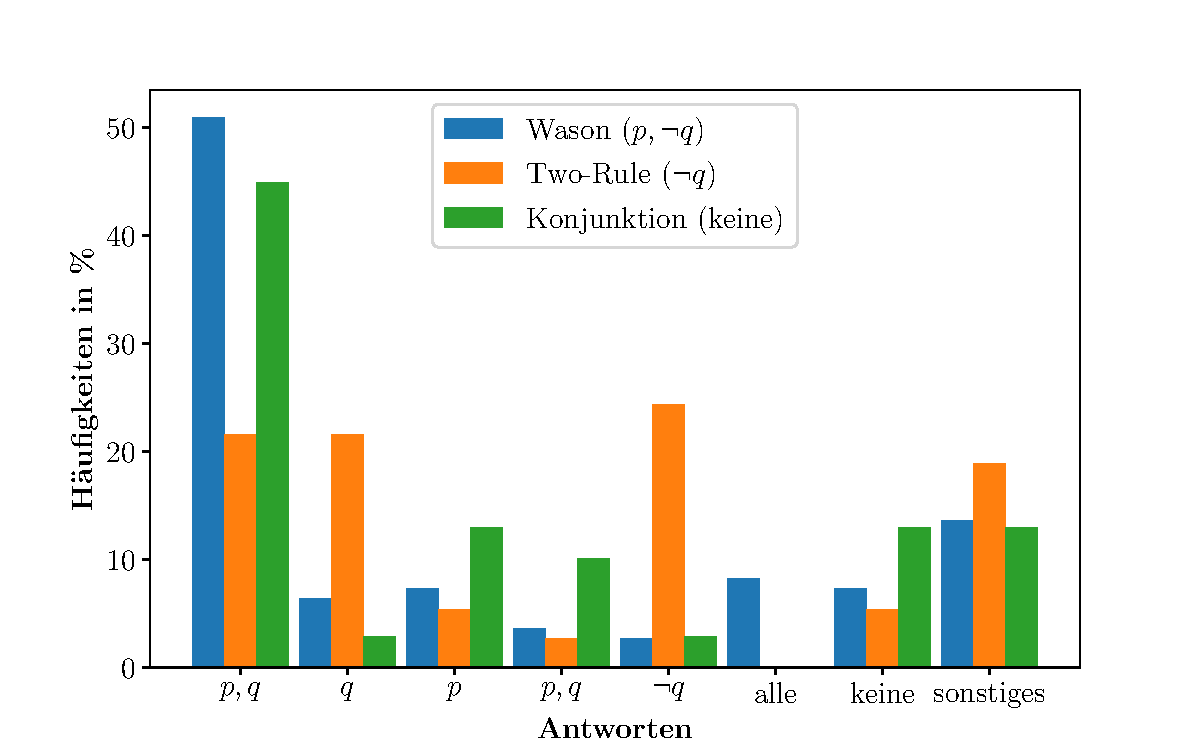
\includegraphics[width=\textwidth]{../plot/results_conjunction.pdf}
\end{frame}


\begin{frame}{Konjunktivisch {\scriptsize \cite[S.~109]{stenningHumanReasoningCognitive2008}}}
    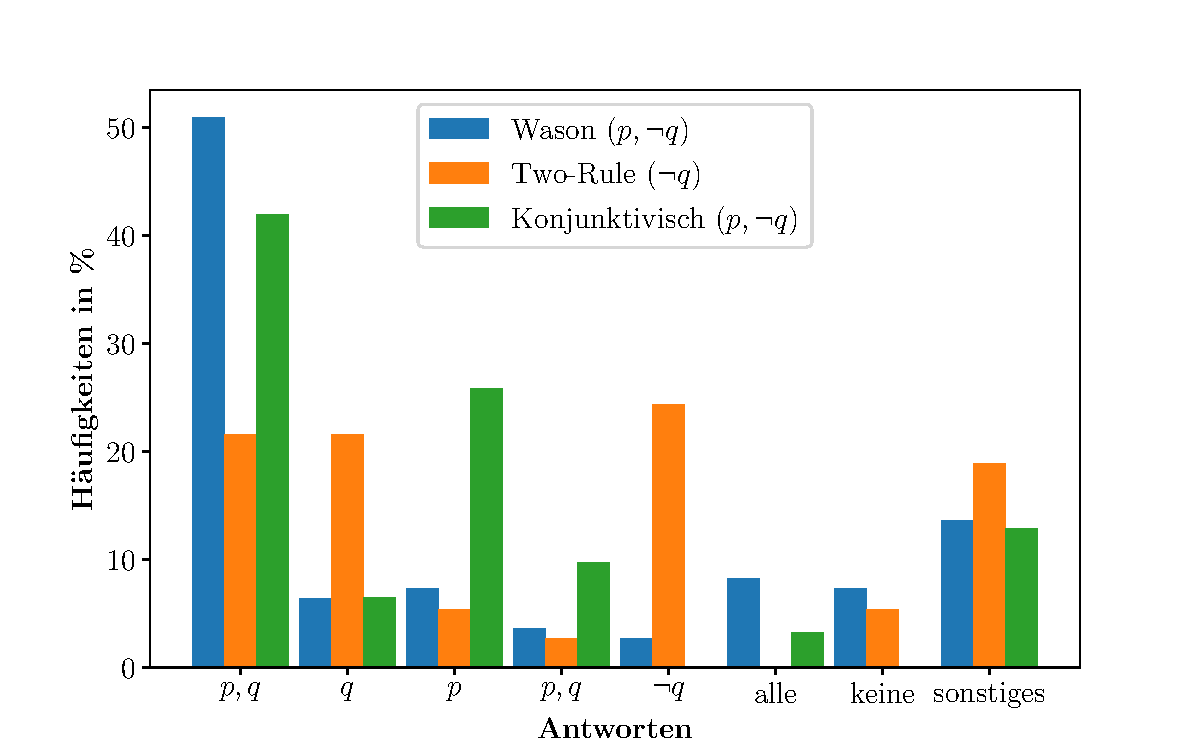
\includegraphics[width=\textwidth]{../plot/results_subjunctive.pdf}
\end{frame}
